%!TEX root = ../master.tex
\chapter{Visualizer}
\label{appendix:visualizer}

The Tangible Cloud Computing cluster is a learning object in itself, it provides hands-on experience with the actual hardware and the possibility of simulating network failures. However it can be hard to understand and grasp what is actually going on in Kubernetes. You can get all the information using the command-line tool: kubectl. But it's way harder to understand the concepts and connections made without having them visualized. Brendan Burns co-founder of the Kubernetes project have created a visualization tool, this tool has been open sourced an build on top of by amongst others, Ray Tsang (saturnism) and Arjen Wassink (awassink). We have forked there repository and added and clean-up the application. The visualizer can be seen in Figure~\ref{fig:visualizer} (a) shows the layout of the application; (b) shows a Rolling-update in progress. 
\begin{figure}[H]%
    \centering
    \subfloat[Simple visualization]{{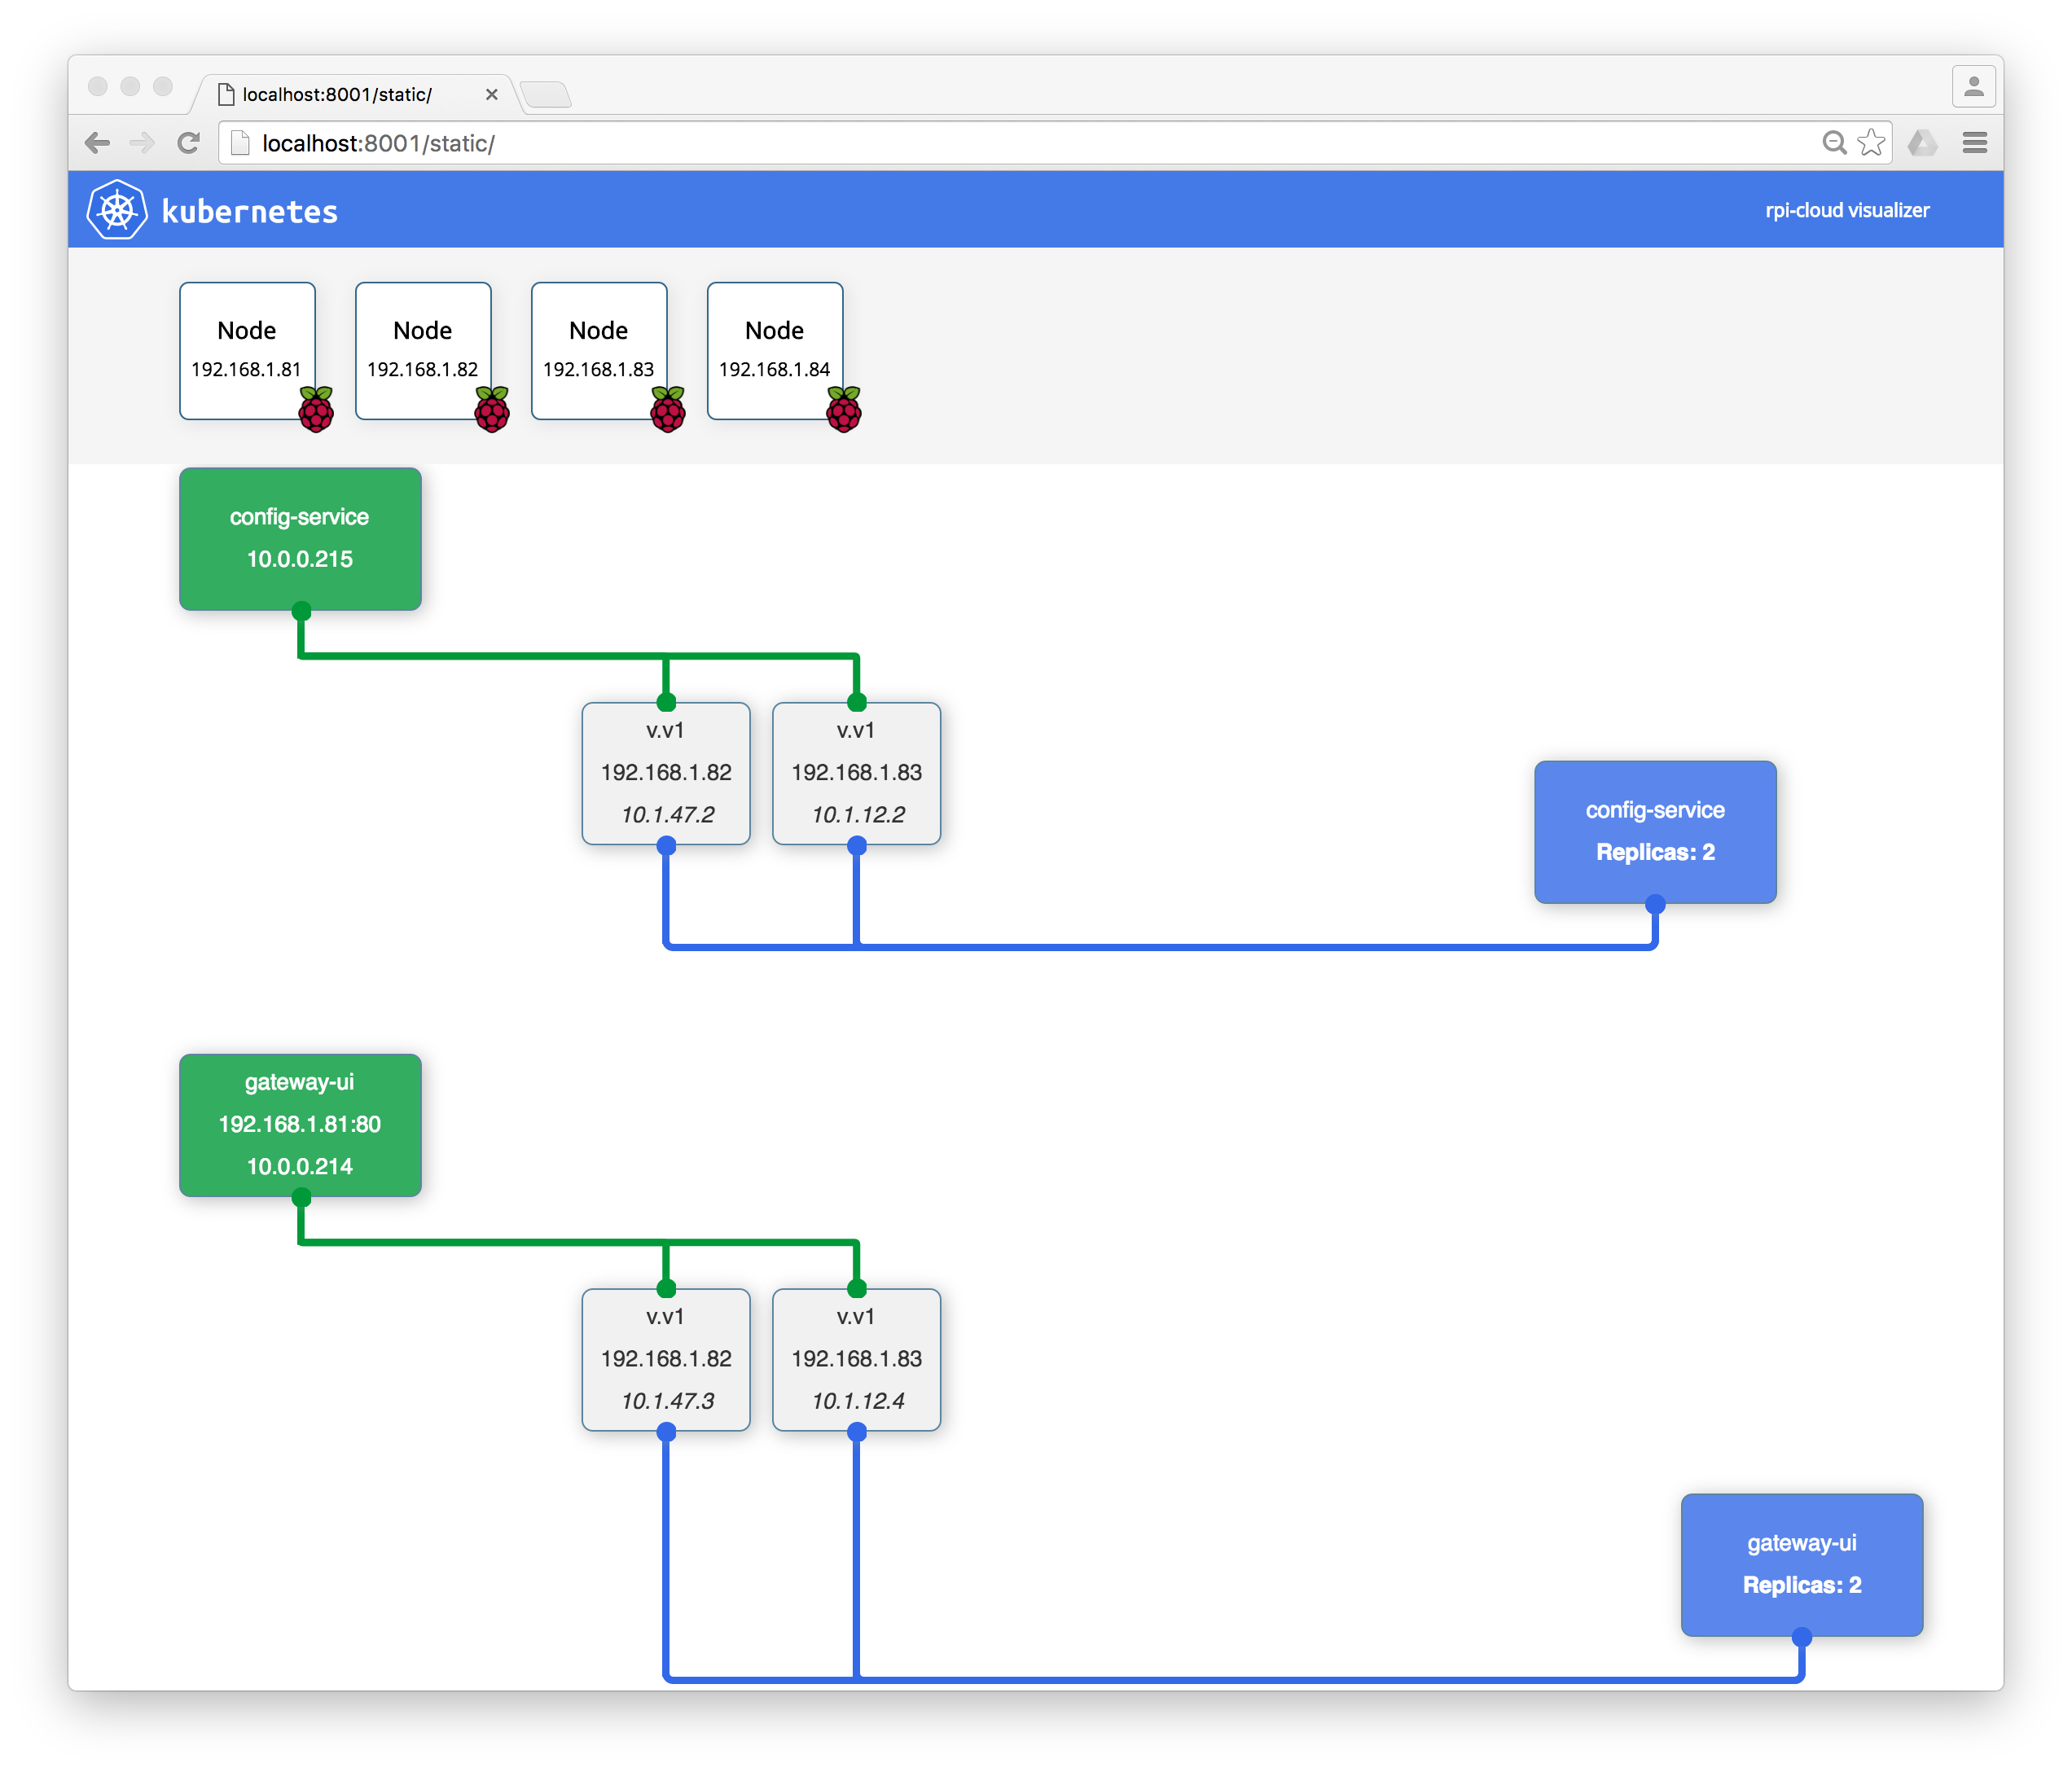
\includegraphics[width=7cm]{figures/visualizer/visualize} }}%
    \qquad
    \subfloat[Rolling update]{{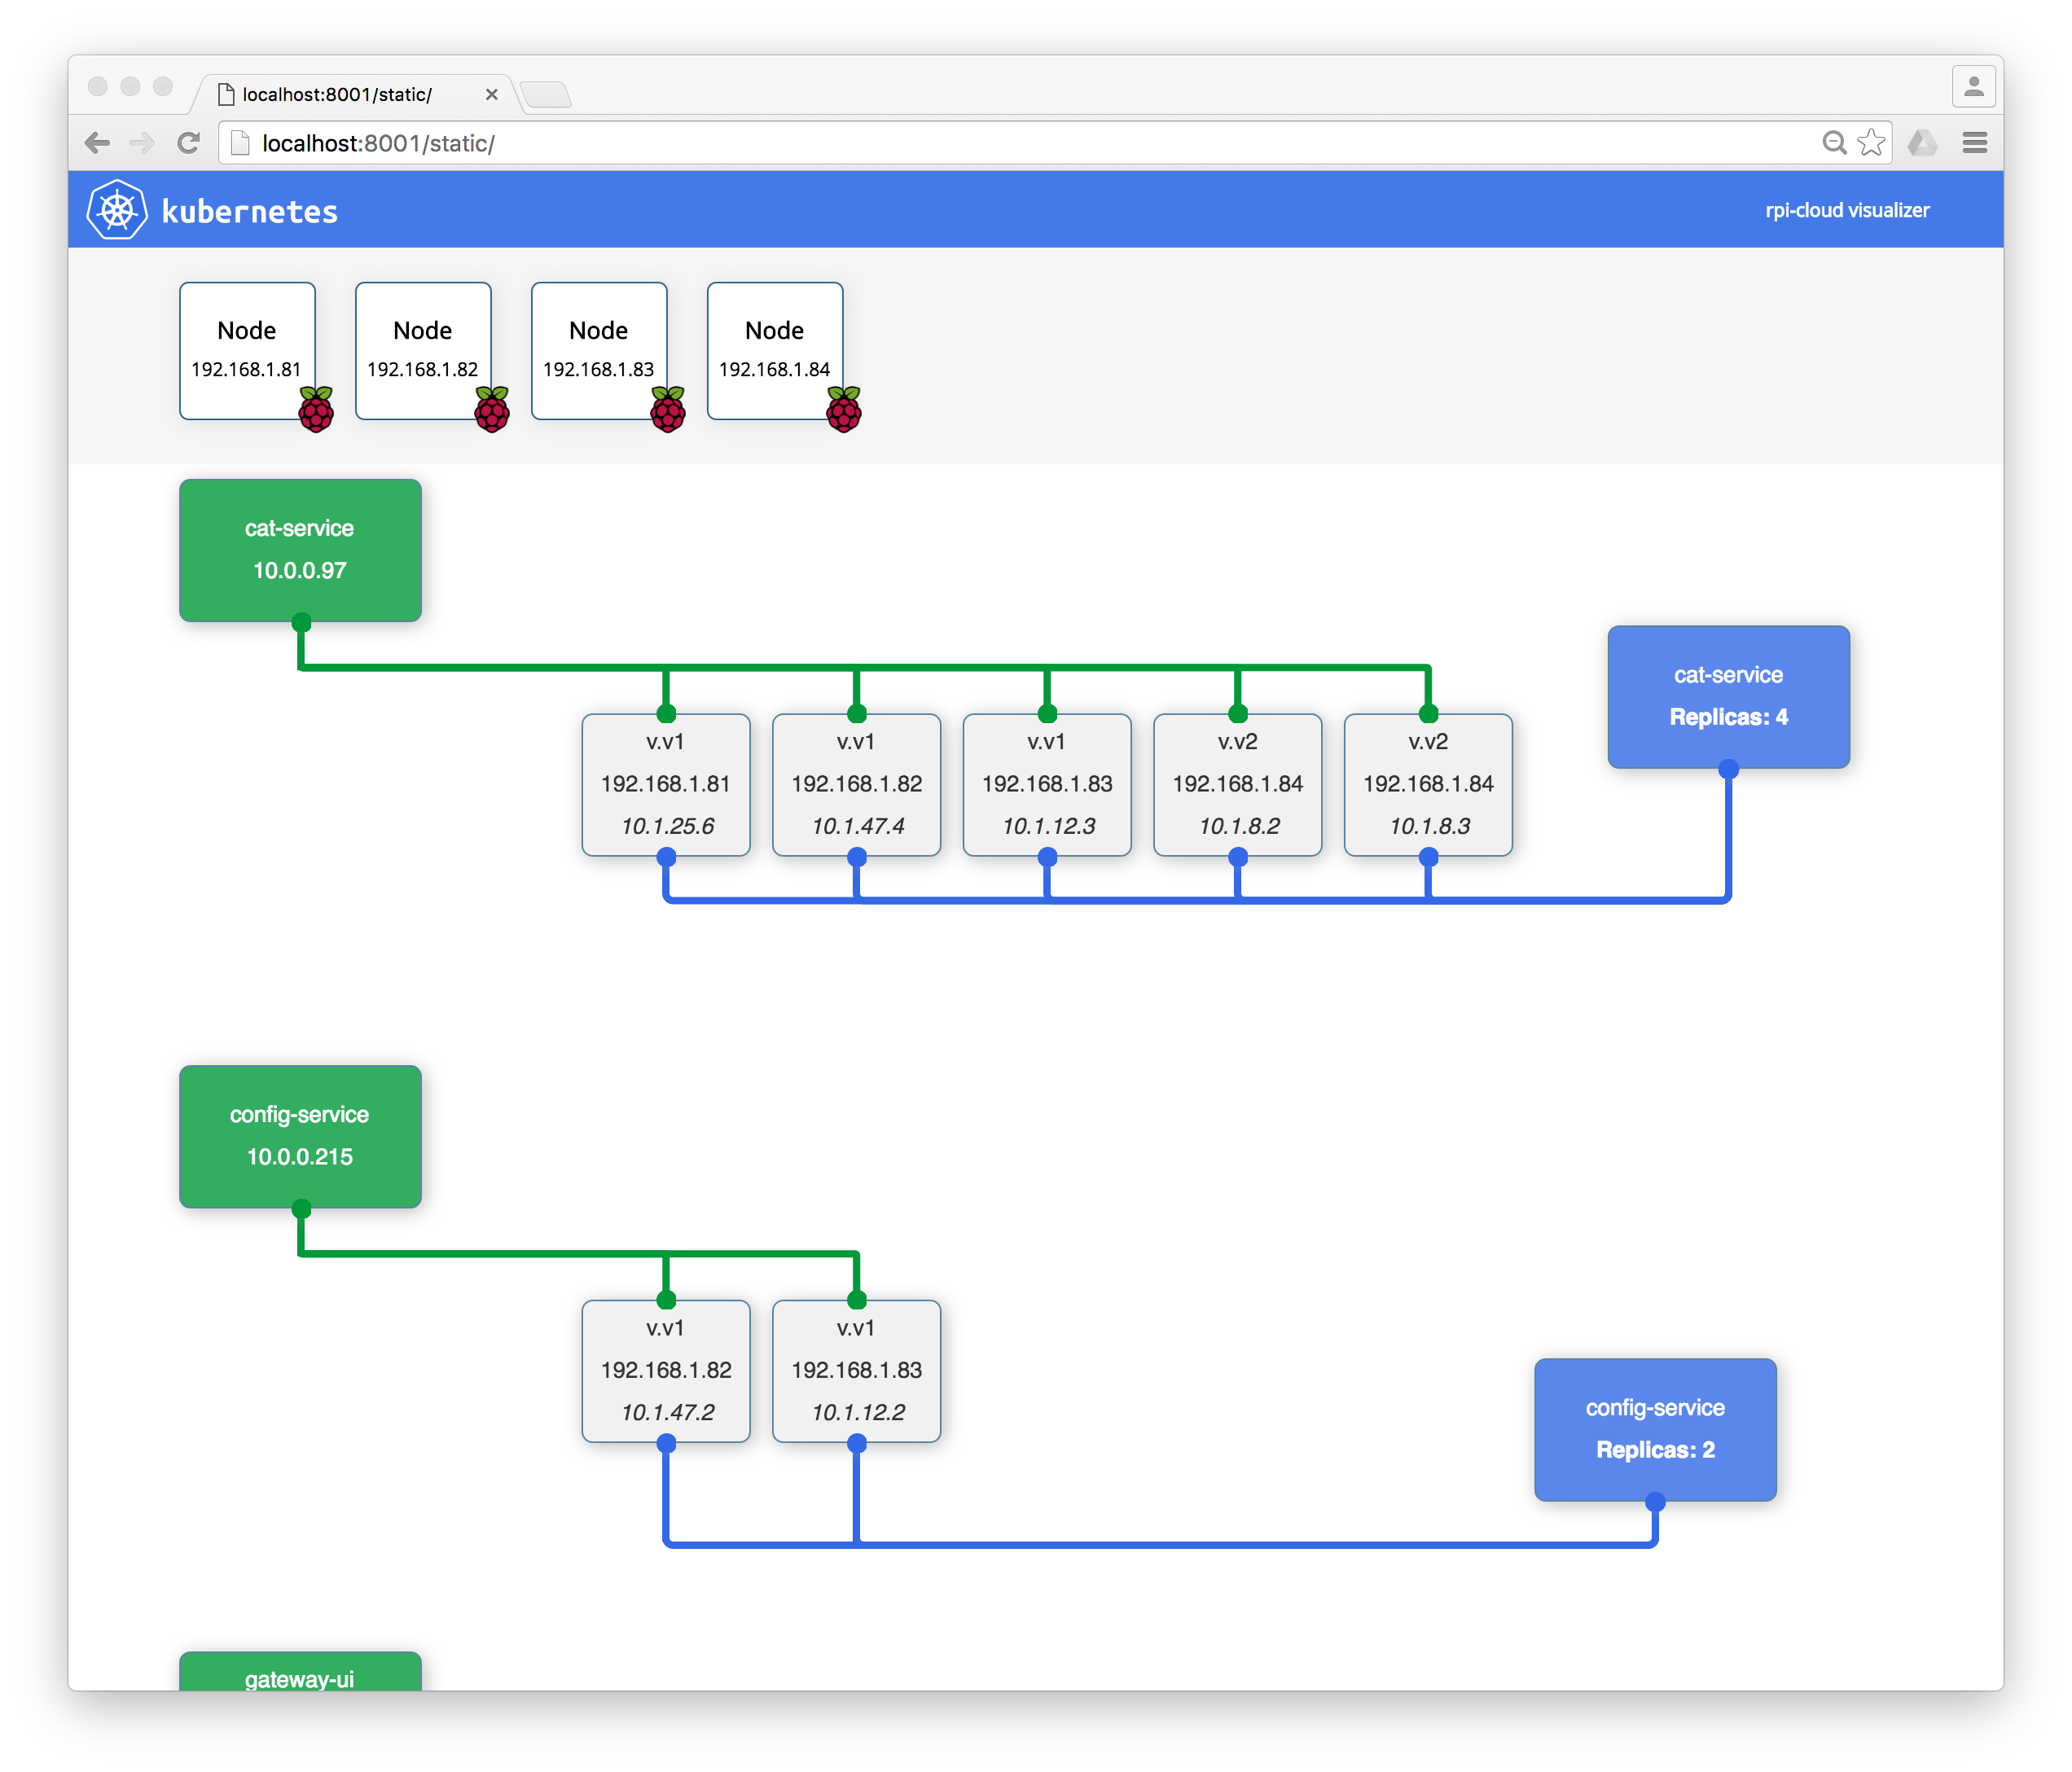
\includegraphics[width=7cm]{figures/visualizer/rolling_update} }}%
    \caption{Screenshots of Visualizer}%
    \label{fig:visualizer}%
\end{figure}

\noindent The 4 white icons shown in the upper bar represents each node in the cluster. A little Raspberry Pi logo have been added, to make the connection between the visualizer tool and the tangible cloud computing cluster more clear. The grey squares connected by blue and green lines represents Pods in Kubernetes. The blue square represents a deployment and the green represents a service, and the load-balancing aspects of the service visually easy to see. Concepts like rolling-updates is fairly easy understood when visualized. We have added the specific version to each Pod, making it more clear how far along in the rolling-update progression Kubernetes is. Another improvement to the tool we have made, is the ability to more clearly visualize what happens when a node is removed from the network. Figure~\ref{fig:visualizer_node_failure} demonstrates a scenario where we pull the plug of the node to the most right. Kubernetes detects this an set the status to NotReady, the application polls the Kubernetes API every 3 seconds and when the NotReady status is received the node is marked with Red (a). Kubernetes then reschedules (b) the Pods that was running on the failing node, this is again visualized with red color, and the Pods being started are visualized with Yellow, while there status is Pending. When the newly scheduled Pod is ready it changes color back to the original color (c). Lastly when Kubernetes have cleaned up after the node failure, everything is running as normal, and the deployment still have the desired level of 3 Pods running.

\begin{figure}[H]%
    \centering
    \subfloat[Node failure]{{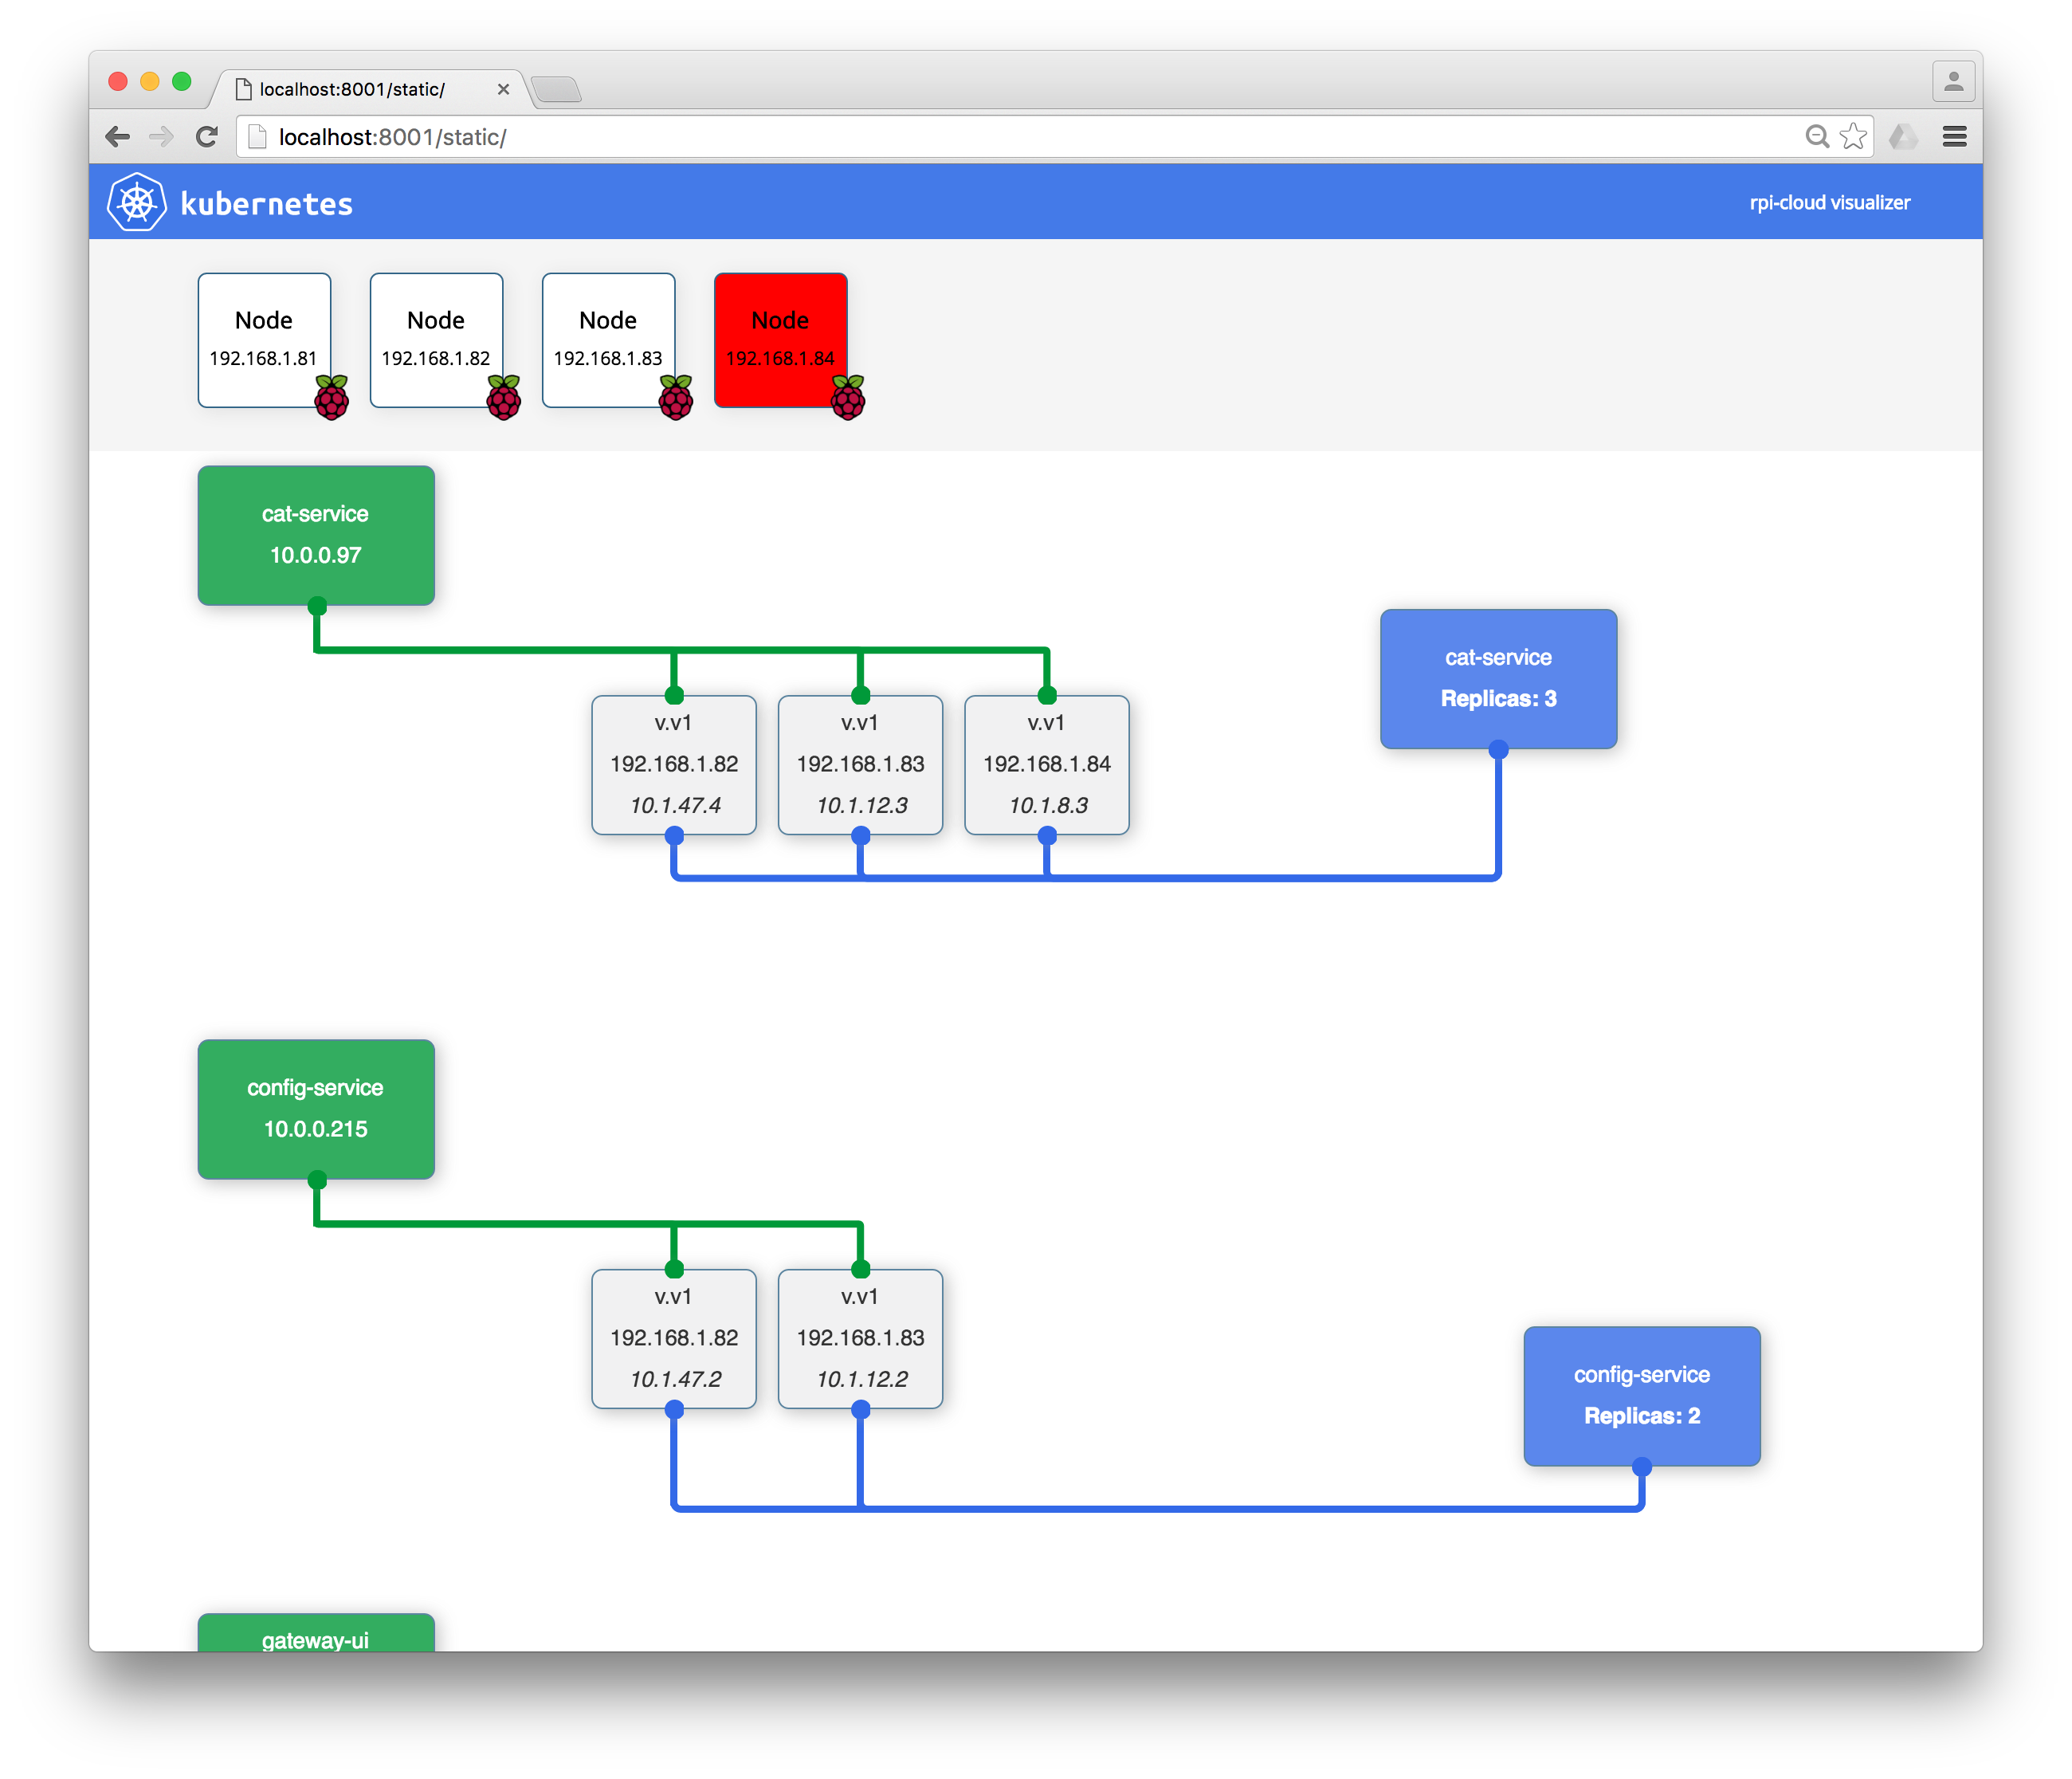
\includegraphics[width=7cm]{figures/visualizer/node_fail} }}%
      \qquad
    \subfloat[Rescheduling]{{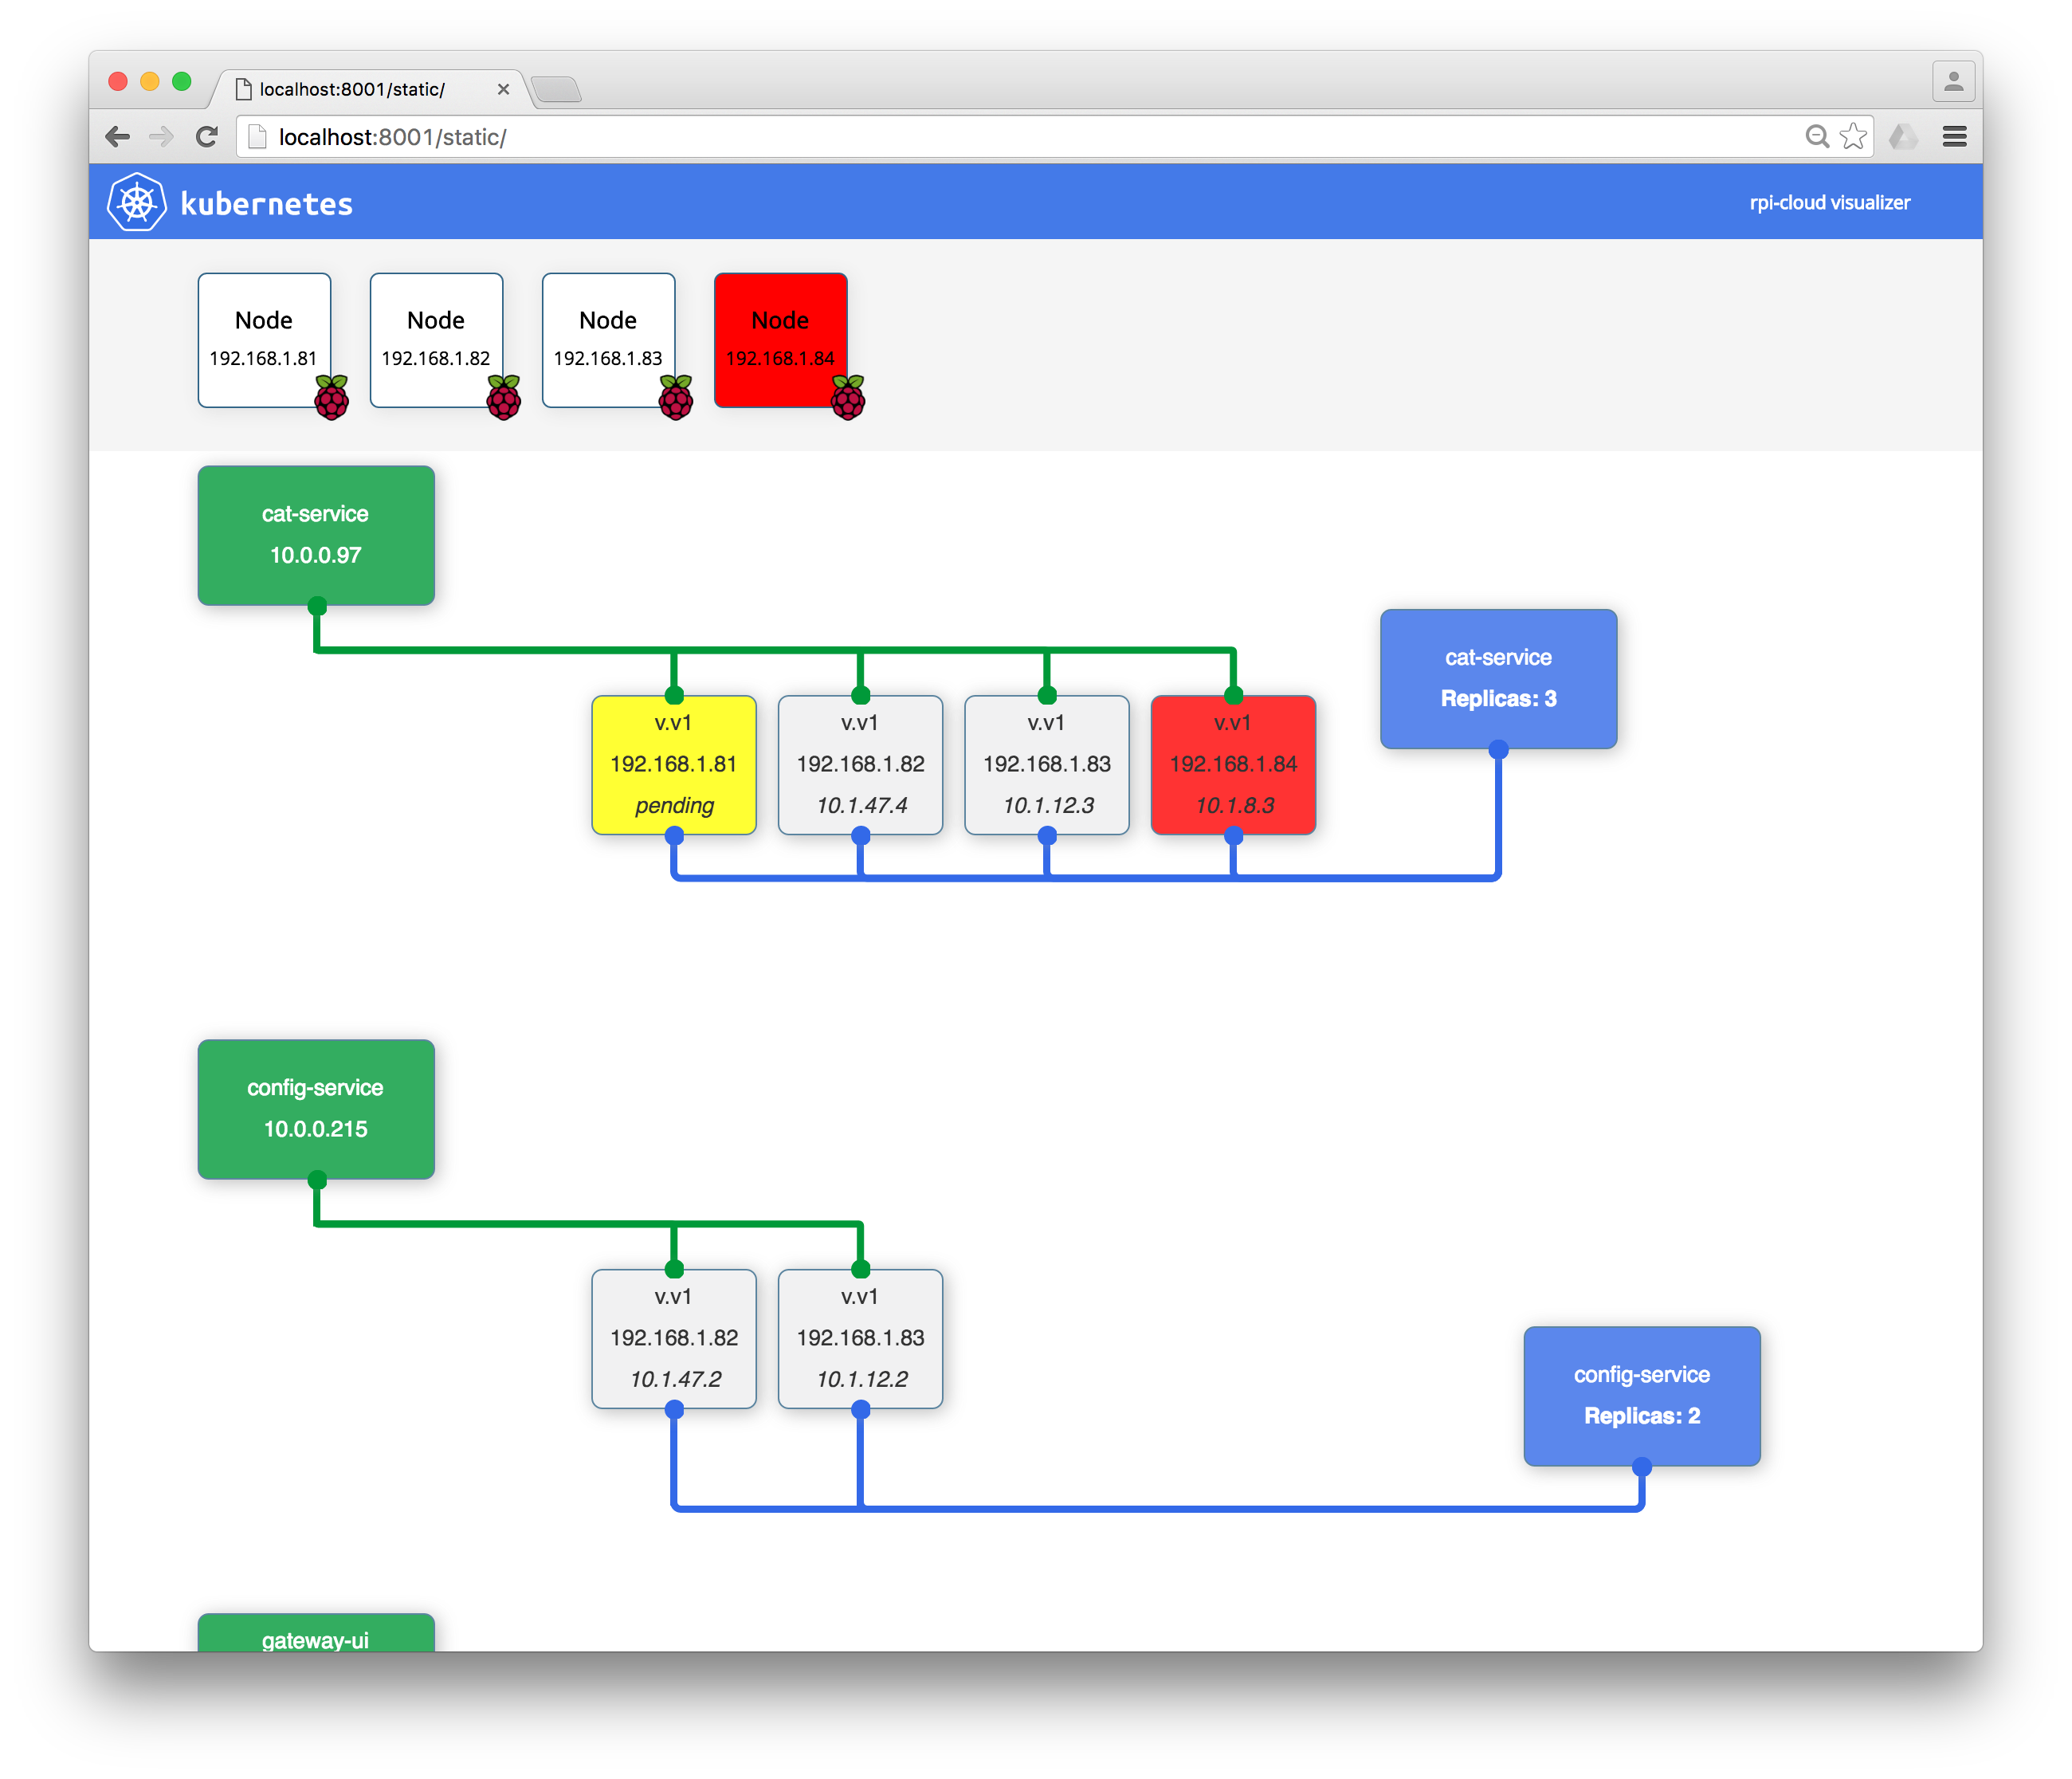
\includegraphics[width=7cm]{figures/visualizer/node_fail_reschedule} }}%
          \qquad
    \subfloat[Clean up]{{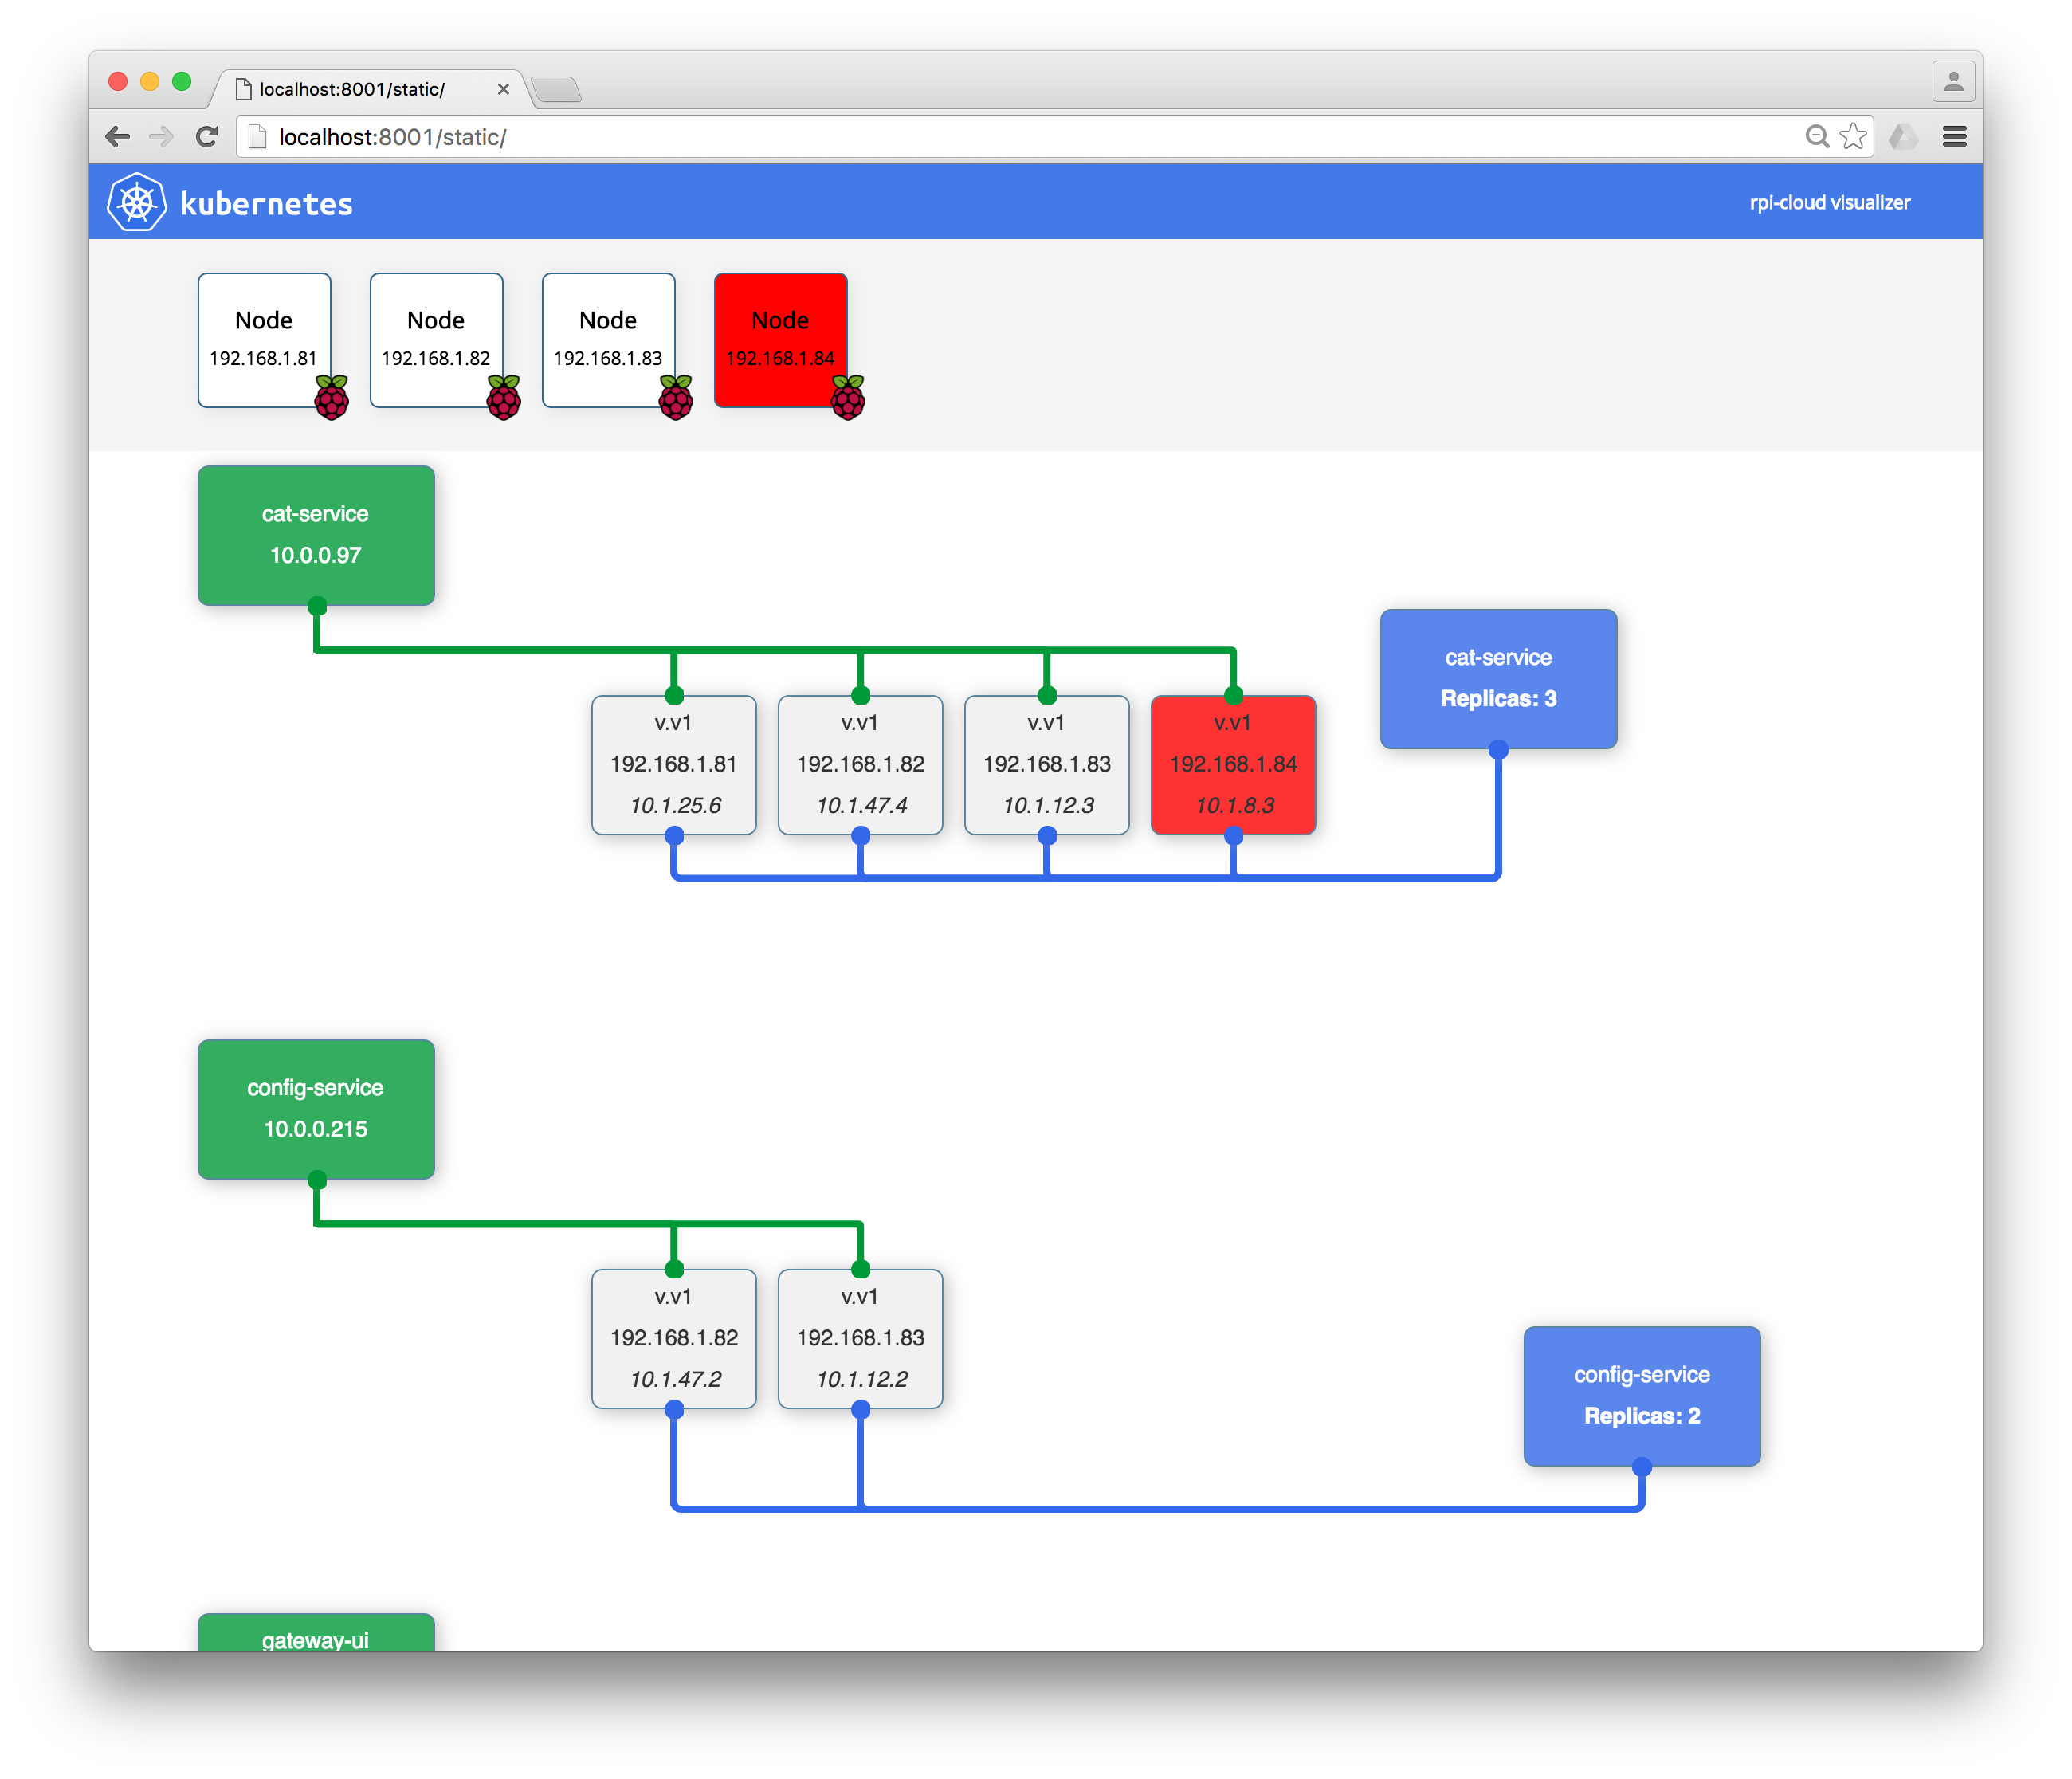
\includegraphics[width=7cm]{figures/visualizer/node_fail_clean_up} }}%
          \qquad
    \subfloat[Recovered]{{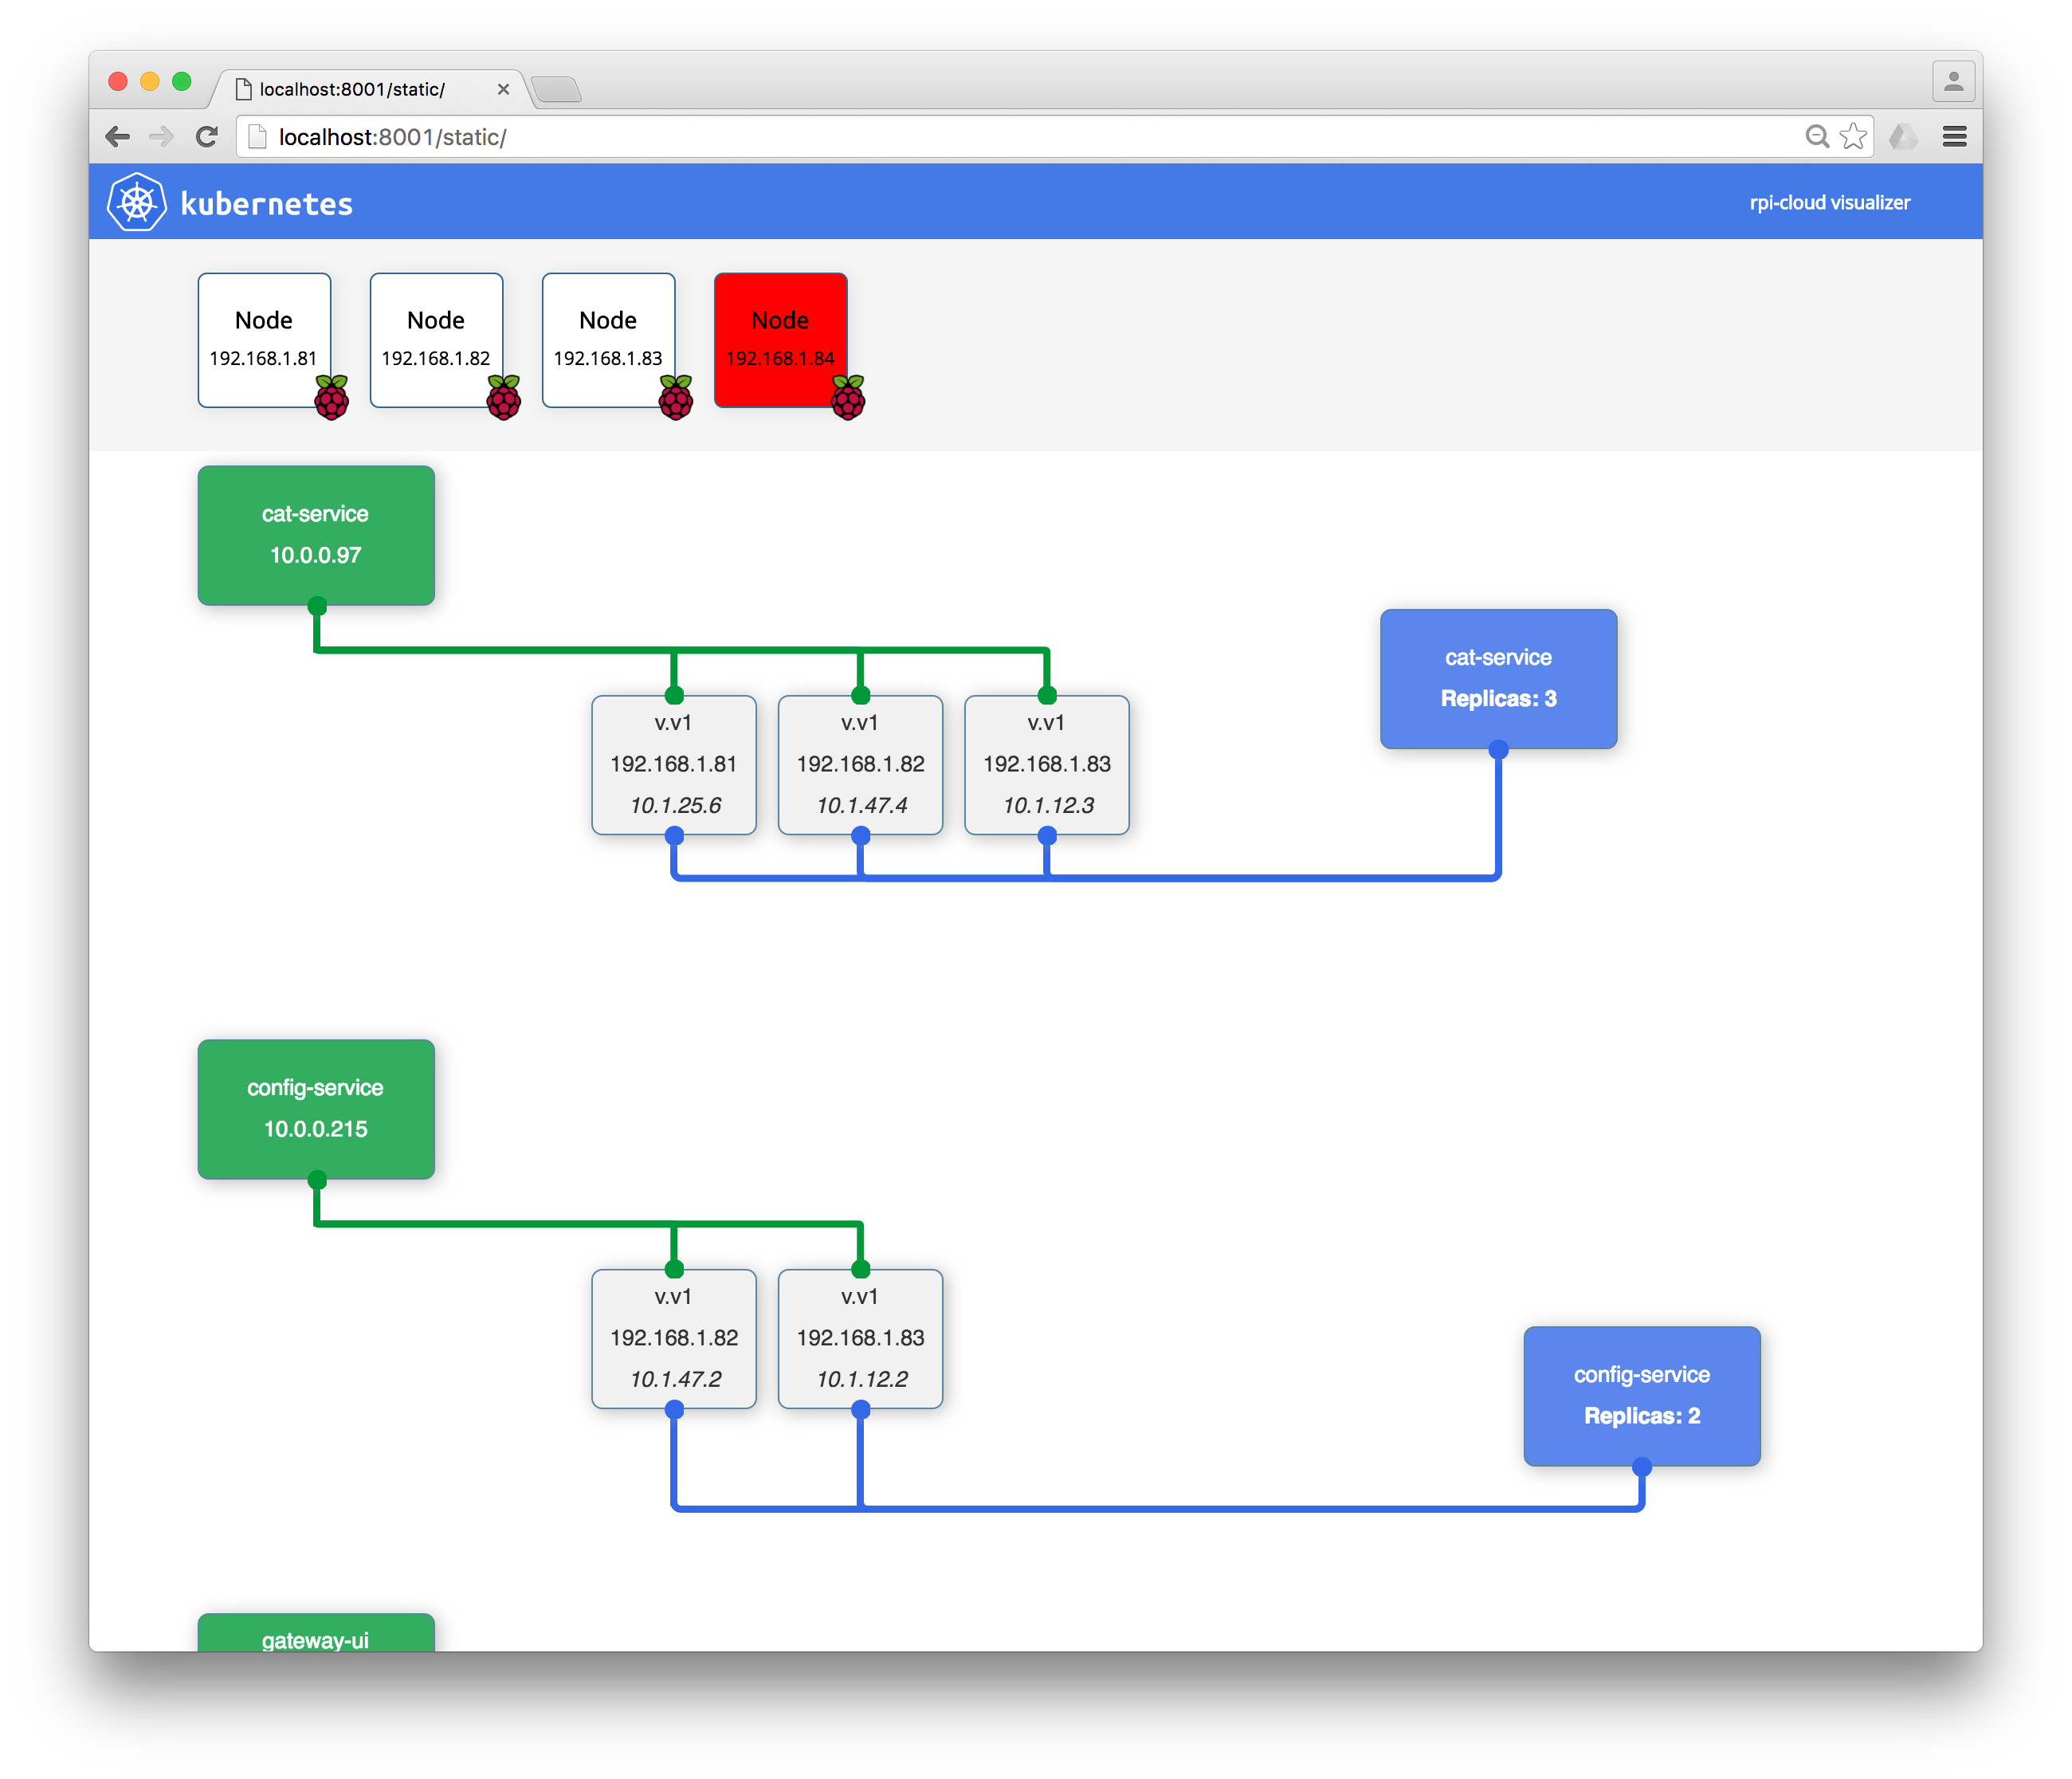
\includegraphics[width=7cm]{figures/visualizer/node_fail_recovered} }}%
    \caption{Visualization of Node failure}%
    \label{fig:visualizer_node_failure}%
\end{figure}

\noindent Further improvements to the visualizer made during this master thesis are among others fixing a memory leak in the original code. The drawing of nodes in the DOM, kept being overlayed every 3 seconds. The result of having the visualizer open for longer periods made it heavy to interact with because of the addition of basically the same DOM elements, instead of re-drawing og cleaning up before drawing. Further the introduction of Kubernetes 1.2 brought some problems, because of the introduction of new concepts, like deployments instead of ReplicaControllers. The visualizer was modified to work Kubernetes 1.2.
